% ████████████████████████████████████████████████████████████████████████████████
%
%   CODEX ΔΦ — CYBERNETIC MEMORY SYSTEM SOFTWARE ARCHITECTURE
%   (CMS-SA v0.1)
%   ────────────────────────────────────────────────────────────────────────────
%   MINIMAL RUNNABLE CYBERNETIC MEMORY RUNTIME, CMS v1.0/v1.1 THEORY BRIDGE,
%   OBSERVATION/METRIC/COMPARATOR/FEEDBACK LIFECYCLE EXECUTION, DRIFT
%   DECOMPOSITION, CONTROL-UTILITY MEMORY PROMOTION, README/RCC/PUBLIC-SURFACE
%   DRIFT GUARDS, ADOPTION PROFILE CHECKS, BASELINE UTILITY TASKS, EVIDENCE
%   PACKAGE GENERATION, RCC NEXUS NAVIGATION, AND ROOTMIRROR-READY ARTIFACT
%   EMISSION WITHOUT CLAIMING AUTONOMOUS INTELLIGENCE, CONSCIOUSNESS, AGI,
%   MODEL-WEIGHT SELF-MODIFICATION, EMPIRICAL TRUTH, OR REAL-WORLD CORRECTNESS
%
%   VERSION
%   ───────
%   v0.1 — Minimal Runtime Genesis and Cybernetic Memory Execution Layer · Locked ·
%          CMS v1.0/v1.1 Runtime Bridge, CyberneticState Contract,
%          MetricContract Contract, DriftReport Contract, FeedbackItem Contract,
%          FeedbackLifecycle Engine, NextVersionPlan Contract, ValidationReport,
%          MemoryCandidate Contract, ControlUtilityPromotion Gate,
%          SurfaceAlignment Audit, PublicSurfaceDrift Guard, CorrectionRecord,
%          ReleaseSeal, BaselineUtility Harness, EvidencePackage, CLI,
%          README_90_SECONDS.md, RCC Nexus Mini-READMEs, Tests, Visuals, and
%          RootMirror-Ready Output Grammar
%
%   AUTHOR
%   ──────
%   James Paul Jackson
%   X / Twitter: @unifiedenergy11
%
%   SOURCE / AUTHOR ATTRIBUTION
%   ───────────────────────────
%   This document is a Codex-format software architecture derived from and
%   aligned with:
%
%       • CODEX ΔΦ — CYBERNETIC MEMORY SYSTEM (CMS v1.0), especially:
%           (1) cybernetic memory loop,
%           (2) memory-as-control-surface definition,
%           (3) feedback signal algebra,
%           (4) comparator and drift,
%           (5) versioned self-improvement,
%           (6) RCC Nexus integration,
%           (7) evidence-of-utility requirement,
%           (8) correction-is-not-deletion rule.
%
%       • CODEX ΔΦ — CYBERNETIC MEMORY SYSTEM (CMS v1.1), especially:
%           (1) metric contracts,
%           (2) feedback lifecycle state machine,
%           (3) drift decomposition,
%           (4) control-utility memory promotion,
%           (5) README/RCC narrative-surface drift guard,
%           (6) public-surface drift guard,
%           (7) adoption profiles,
%           (8) baseline utility protocol.
%
%       • CODEX ΔΦ — TAU SCALING SOFTWARE ARCHITECTURE
%         (TAU-SCALING-SA v0.1), used here as the software-architecture
%         formatting, runtime-loop, repository-grammar, evidence-package,
%         CLI, roadmap, validation/falsification, and non-claim process
%         template.
%
%       • Tau Scaling repository lessons, especially:
%           (1) Human README / RCC Nexus README / AI Agent README trisection,
%           (2) README + mini README audit map,
%           (3) AI failure-learning ledger,
%           (4) release validator as final local gate,
%           (5) source/evidence intake discipline,
%           (6) primary-source validation gap review,
%           (7) public release candidate packaging,
%           (8) mismatch risk between local/uploaded/public repository states.
%
%       • Codex CITA / CIF / CEM / RCC / CIK / AERMA / RootMirror operating
%         lessons:
%           raw insight must become governed artifact;
%           governed artifacts must expose validation surfaces;
%           validation surfaces must prevent claim inflation;
%           memory promotion must preserve reusable invariants only;
%           README/RCC drift is repository drift;
%           public narrative surfaces must match current artifact state;
%           local anchoring and artifact emission precede release.
%
%   CMS v1.1 extracted the software-relevant invariant:
%
%       A cybernetic memory system improves only when feedback becomes a typed,
%       measured, lifecycle-tracked control signal that changes a bounded next
%       version, survives validation, preserves correction history, and updates
%       human-readable, RCC-readable, AI-readable, and public repository
%       surfaces.
%
%   CMS-SA v0.1 turns that invariant into a minimal Python/RCC software
%   architecture. It does not claim implementation completion, autonomous
%   intelligence, consciousness, AGI, empirical truth, real-world correctness,
%   model-weight self-modification, or proof that repository feedback is
%   sentience.
%
%   Short repo name:
%
%       cybernetic-memory-system
%
%   Python package / CLI name:
%
%       cms
%
%   DATE
%   ────
%   May 2026
%
%   STATUS
%   ──────
%   CANONICAL v0.1 SOFTWARE ARCHITECTURE GENESIS LAYER —
%   NOT IMPLEMENTED YET · NOT A REPLACEMENT FOR CMS v1.0/v1.1 · NOT AUTONOMOUS
%   INTELLIGENCE · NOT CONSCIOUSNESS · NOT AGI · NOT MODEL-WEIGHT SELF-
%   MODIFICATION · NOT EMPIRICAL TRUTH · NOT PROOF THAT VALIDATION EQUALS
%   REAL-WORLD CORRECTNESS · NOT A CLAIM THAT REPOSITORY FEEDBACK IS SENTIENCE ·
%   NOT PERMISSION TO PROMOTE MEMORY WITHOUT CONTROL UTILITY, SOURCE BOUNDARY,
%   VALIDATION, NON-CLAIM SAFETY, AND CORRECTION COMPATIBILITY
%
%   PURPOSE
%   ───────
%   Define the software architecture for a minimal Cybernetic Memory System
%   runtime that turns CMS v1.0/v1.1 from canonical feedback-memory theory into
%   executable software:
%
%       repository state / prior memory / public surfaces
%       → observation manifest
%       → metric contracts
%       → drift decomposition
%       → typed feedback items
%       → feedback lifecycle resolution
%       → next-version plan
%       → validation report
%       → control-utility memory scoring
%       → correction record
%       → surface-alignment audit
%       → release seal
%       → evidence package
%       → RCC/AI/public routing surfaces.
%
%   WHAT THIS IS
%   ────────────
%   • A software architecture for executable cybernetic repository memory
%   • A minimal Python package design
%   • A governed CLI architecture
%   • An executable CMS v1.0/v1.1 runtime-loop design
%   • A metric-contract and drift-decomposition architecture
%   • A feedback lifecycle and next-version planning architecture
%   • A control-utility memory-promotion architecture
%   • A README/RCC/public-surface drift guard architecture
%   • A correction-record and release-seal architecture
%   • A baseline utility harness architecture
%   • An evidence package, dashboard, and report architecture
%   • A README_90_SECONDS.md adoption layer
%   • A RootMirror-ready local artifact grammar
%
%   WHAT THIS IS NOT
%   ───────────────
%   • Not an implemented repository yet
%   • Not a replacement for CMS v1.0/v1.1
%   • Not a claim of AGI
%   • Not a claim of consciousness
%   • Not autonomous self-modification
%   • Not model-weight modification
%   • Not proof that feedback is true
%   • Not proof that validation equals real-world correctness
%   • Not permission to promote memory without control utility
%   • Not permission to release when local, uploaded, generated, and public
%     surfaces disagree
%   • Not permission to treat README/RCC alignment as code correctness
%
%   CORE EXTRACTION
%   ───────────────
%   CMS-SA v0.1 extracts the software invariant:
%
%       Cybernetic repository memory becomes useful only when it becomes
%       executable, auditable, metric-declared, drift-decomposed, feedback-
%       lifecycle-tracked, validation-bound, control-utility-promoted,
%       correction-preserving, surface-aligned, evidence-packaged, and
%       release-gated.
%
%   First target runtime:
%
%       CMS v0.1 Minimal Runtime
%
%   First target seeds:
%
%       cms-lite-self-audit-seed
%       readme-rcc-drift-seed
%       feedback-lifecycle-seed
%       memory-promotion-seed
%       baseline-utility-seed
%       public-surface-drift-seed
%
%   First admissible CMS release functional:
%
%       A_CMS = B_state B_metric B_drift B_feedback B_lifecycle B_plan
%               B_validation B_memory B_correction B_surface B_public
%               B_release (1 - O)
%
%   CANONICAL LOCK (v0.1)
%   ─────────────────────
%   • CMS-SA implements CMS v1.0/v1.1; it does not replace CMS v1.0/v1.1.
%   • Feedback is not truth.
%   • Memory is not consciousness.
%   • Self-improvement is versioned artifact improvement.
%   • Validation is repository-bound unless external evidence is supplied.
%   • Control utility is required for memory promotion.
%   • Correction is not deletion.
%   • Drift is not evolution unless validated.
%   • README/RCC drift is repository drift.
%   • Public-surface drift is release drift.
%   • Surface alignment is not code correctness.
%   • Baseline utility claims require baseline comparison.
%   • Release is bounded actuation.
%
%   RCC INJECTION LOCK (v0.1)
%   ─────────────────────────
%   The repository must be human/AI readable from genesis:
%
%       root README
%       → README_90_SECONDS.md
%       → AGENTS.md
%       → rcc/nexus/route_map.json
%       → docs/context/repository_context_index.json
%       → folder mini READMEs
%       → state / metrics / drift / feedback / validation / memory / correction
%         / release / evidence artifacts
%       → public-surface synchronization report.
%
%   SOFTWARE NON-CLAIM LOCK (v0.1)
%   ─────────────────────────────
%   CMS-SA measures and emits cybernetic repository-memory governance artifacts.
%   It does not prove consciousness, intelligence, truth, code correctness,
%   external validation, production safety, provenance, model self-modification,
%   or real-world empirical correctness.
%
%   AI PROMPT TRACEABILITY
%   ──────────────────────
%   Use this document as the canonical CMS-SA v0.1 software architecture
%   genesis layer. Preserve CMS v1.0/v1.1 as host theory/evidence bridge.
%   Implement only a minimal runtime first: repository observation, metric
%   contracts, decomposed drift report, typed feedback report, lifecycle state
%   transitions, next-version plan, validation report, control-utility memory
%   promotion, correction record, surface-alignment audit, public-surface drift
%   guard, release seal, evidence JSON, reports, logs, tests, README_90_SECONDS,
%   RCC route map, and mini READMEs.
%
%   SHADOW HEADER ALIGNMENT SEAL
%   ───────────────────────────
%   Preserve header discipline across future CMS-SA versions except for
%   explicitly additive refinements that improve implementation readiness,
%   runtime auditability, source fidelity, metric contracts, feedback lifecycle,
%   drift decomposition, memory promotion, validation, surface alignment,
%   evidence packaging, CLI usability, test coverage, or public engineering
%   clarity.
%
% ████████████████████████████████████████████████████████████████████████████████

\documentclass[12pt]{article}

\usepackage[margin=1in]{geometry}
\usepackage[utf8]{inputenc}
\usepackage[T1]{fontenc}
\usepackage{amsmath,amssymb,amsfonts,amsthm}
\usepackage{booktabs,longtable,array}
\usepackage{hyperref}
\usepackage{enumitem}
\usepackage{listings}
\usepackage{xcolor}
\usepackage{tikz}
\usetikzlibrary{arrows.meta,positioning,shapes.geometric,fit,calc}

\hypersetup{
  colorlinks=true,
  linkcolor=blue,
  urlcolor=blue,
  citecolor=blue
}

\newtheorem{axiom}{Axiom}
\newtheorem{definition}{Definition}
\newtheorem{proposition}{Proposition}
\newtheorem{requirement}{Requirement}
\newtheorem{remark}{Remark}
\newtheorem{corollary}{Corollary}
\newtheorem{law}{Law}

\lstset{
  basicstyle=\ttfamily\small,
  breaklines=true,
  columns=fullflexible,
  frame=single
}

\title{\textbf{Codex $\Delta\Phi$ --- Cybernetic Memory System Software Architecture (CMS-SA v0.1)}\\
\large Minimal Runtime, Metric Contracts, Feedback Lifecycle, Drift Decomposition, Control-Utility Memory Promotion, Surface Drift Guards, Baseline Utility, and Evidence-Gated Repository Memory}
\author{\textbf{James Paul Jackson}\\[4pt]
\small Codex-format software architecture for executable cybernetic memory governance\\
\small \texttt{@unifiedenergy11}}
\date{May 2026}

\begin{document}
\sloppy
\maketitle

\begin{abstract}
CMS-SA v0.1 defines the software architecture for a minimal Cybernetic Memory
System runtime: a local-first Python/RCC package that operationalizes CMS
v1.0/v1.1 as executable repository-memory governance software. The architecture
converts CMS theory into computable contracts for observation, metrics,
drift decomposition, feedback lifecycle, next-version planning, validation,
control-utility memory promotion, correction history, surface alignment,
baseline utility, release sealing, evidence packaging, and RCC/AI/public
routing. CMS-SA v0.1 is a software architecture, not an implementation claim,
autonomous intelligence, consciousness, AGI, empirical truth, model-weight
self-modification, production-safety guarantee, or proof that repository
validation equals real-world correctness.
\end{abstract}

%──────────────────────────────────────────────────────────────────────────────
\section{Core-Invariant Extraction Block}
%──────────────────────────────────────────────────────────────────────────────

The shortest faithful extraction of CMS-SA v0.1 is:

\begin{center}
\fbox{\begin{minipage}{0.90\textwidth}
CMS-SA turns CMS v1.0/v1.1 into a minimal executable runtime by combining
repository observation, metric contracts, drift decomposition, typed feedback,
feedback lifecycle, next-version planning, validation, control-utility memory
promotion, correction records, surface-alignment audits, public-surface drift
guards, release seals, and evidence packages.
\end{minipage}}
\end{center}

The operative runtime chain is:

\begin{center}
\fbox{\begin{minipage}{0.90\textwidth}
\centering
repo state $\rightarrow$ observation $\rightarrow$ metrics $\rightarrow$ drift
$\rightarrow$ feedback $\rightarrow$ lifecycle $\rightarrow$ plan
$\rightarrow$ validation $\rightarrow$ memory promotion $\rightarrow$
correction $\rightarrow$ surface alignment $\rightarrow$ release seal
$\rightarrow$ evidence package.
\end{minipage}}
\end{center}

CMS-SA v0.1 answers:

\[
\boxed{
\text{How do we make cybernetic repository memory runnable without overclaiming?}
}
\]

\begin{remark}
CMS-SA does not begin by claiming intelligence or autonomy. It begins with the
smallest useful runtime that proves the architecture: observe a repository,
measure declared surfaces, decompose drift, emit lifecycle-tracked feedback,
generate a bounded next-version plan, validate, score memory candidates, preserve
corrections, audit README/RCC/public surfaces, and seal the release.
\end{remark}

%──────────────────────────────────────────────────────────────────────────────
\section{Name and Public Identity}
%──────────────────────────────────────────────────────────────────────────────

\begin{definition}[Cybernetic Memory Runtime]
The Cybernetic Memory Runtime is the minimal software system for observing
repository state, measuring declared metrics, decomposing drift, emitting typed
feedback, resolving feedback through a lifecycle, planning the next version,
validating the plan, promoting only control-useful memory, preserving correction
history, auditing narrative/public surfaces, and emitting a release/evidence
package.
\end{definition}

Recommended repository name:

\begin{lstlisting}
cybernetic-memory-system
\end{lstlisting}

Recommended Python package and CLI name:

\begin{lstlisting}
cms
\end{lstlisting}

Recommended public description:

\begin{quote}
A minimal local-first Python/RCC runtime for cybernetic repository memory:
observe repository state, measure metric contracts, decompose drift, emit and
resolve feedback, plan the next version, validate changes, promote only
control-useful memory, preserve correction history, audit README/RCC/public
surfaces, and emit evidence packages without claiming autonomy, consciousness,
AGI, or truth.
\end{quote}

Short public framing:

\begin{center}
\fbox{\begin{minipage}{0.80\textwidth}
\centering
Observe the repo. Measure the drift. Resolve the feedback.\\
Validate the correction. Promote only useful memory.
\end{minipage}}
\end{center}

%──────────────────────────────────────────────────────────────────────────────
\section{Source Lessons Injected into CMS-SA}
%──────────────────────────────────────────────────────────────────────────────

CMS-SA v0.1 injects nine lessons.

\subsection{CMS v1.0 Lesson: Memory Becomes Cybernetic Only Through Closure}

CMS v1.0 teaches:

\[
Observe\rightarrow Measure\rightarrow Compare\rightarrow Feedback\rightarrow Plan\rightarrow Validate\rightarrow Promote\rightarrow Release.
\]

CMS-SA imports this as:

\[
\boxed{\text{no CMS runtime claim without a closed loop artifact chain.}}
\]

\subsection{CMS v1.1 Lesson: Feedback Must Have a Lifecycle}

CMS v1.1 teaches:

\[
Feedback(F_i)\Rightarrow LifecycleState(F_i)\wedge ResolutionTarget(F_i).
\]

CMS-SA imports this as:

\[
\boxed{\text{no orphan feedback.}}
\]

\subsection{CMS v1.1 Lesson: Vague Usefulness Is Not Enough}

CMS v1.1 teaches:

\[
Promote(m)\Rightarrow P_M(m)\geq\theta_M\wedge ControlUseful(m).
\]

CMS-SA imports this as:

\[
\boxed{\text{no control utility, no memory promotion.}}
\]

\subsection{Tau Scaling Lesson: No Baseline, No Gain}

Tau Scaling teaches:

\[
Claim(Improvement)\Rightarrow BaselineComparison.
\]

CMS-SA imports this as:

\[
\boxed{\text{no baseline, no CMS utility claim.}}
\]

\subsection{Tau Scaling Lesson: Human/RCC/AI Trisection Is Operational}

Tau Scaling teaches that a repo must separate:

\[
HumanREADME+RCCNexusREADME+AIAgentREADME.
\]

CMS-SA imports this as:

\[
\boxed{\text{no surface alignment without human, RCC, and AI routing surfaces.}}
\]

\subsection{Tau Scaling Lesson: Failure Must Become Durable Learning}

Tau Scaling's AI failure-learning ledger teaches:

\[
Failure\rightarrow RootCause\rightarrow PermanentRule.
\]

CMS-SA imports this as:

\[
\boxed{\text{failed correction becomes memory only when compressed into a reusable rule.}}
\]

\subsection{RCC Lesson: Context Drift Is System Drift}

RCC teaches:

\[
RouteMapStale\vee MiniREADMEStale\Rightarrow AgentRisk.
\]

CMS-SA imports this as:

\[
\boxed{\text{README/RCC drift is repository drift.}}
\]

\subsection{Public Release Lesson: Local State Can Diverge From Public State}

The Tau Scaling upload/public mismatch lesson teaches:

\[
LocalCurrent\not\Rightarrow PublicCurrent.
\]

CMS-SA imports this as:

\[
\boxed{\text{public-surface drift is release drift.}}
\]

\subsection{Codex Lesson: Release Is Bounded Actuation}

Codex release discipline teaches:

\[
Release\Rightarrow State\wedge Validation\wedge Ledger\wedge SurfaceAlignment.
\]

CMS-SA imports this as:

\[
\boxed{\text{no release seal without validation and surface alignment.}}
\]

%──────────────────────────────────────────────────────────────────────────────
\section{CMS-SA System Definition}
%──────────────────────────────────────────────────────────────────────────────

CMS-SA v0.1 is:

\[
\mathcal{CSA}
=
\{K,O,M,C,D,F,L,P,V,U,R,A,B,E,Q\}.
\]

where:

\[
K=\text{runtime kernel},\quad
O=\text{observation engine},\quad
M=\text{metric contract engine},\quad
C=\text{comparator},
\]

\[
D=\text{drift decomposition engine},\quad
F=\text{feedback generator},\quad
L=\text{feedback lifecycle engine},
\]

\[
P=\text{next-version planner},\quad
V=\text{validation engine},\quad
U=\text{control-utility promotion engine},
\]

\[
R=\text{correction recorder},\quad
A=\text{surface-alignment auditor},\quad
B=\text{baseline utility harness},
\]

\[
E=\text{evidence writer},\quad
Q=\text{release classifier}.
\]

The minimal runtime target is:

\[
\begin{aligned}
\mathcal{CSA}_{v0.1}=\{&
\text{repository observation},\text{metric contracts},\text{drift report},
\text{typed feedback},\\
&\text{feedback lifecycle},\text{next-version plan},\text{validation report},
\text{memory promotion score},\\
&\text{correction record},\text{surface alignment audit},
\text{release seal},\text{evidence package}\}.
\end{aligned}
\]

%──────────────────────────────────────────────────────────────────────────────
\section{Mathematical Runtime Core}
%──────────────────────────────────────────────────────────────────────────────

\subsection{Admissible CMS Release Functional}

The runtime centers on:

\[
\boxed{
\mathcal{A}_{CMS}
=
B_sB_mB_dB_fB_lB_pB_vB_uB_cB_aB_{pub}B_r(1-O).
}
\]

Each term is bounded:

\[
B_s,B_m,B_d,B_f,B_l,B_p,B_v,B_u,B_c,B_a,B_{pub},B_r,O\in[0,1].
\]

where:

\[
B_s=\text{state observed},\quad
B_m=\text{metric contracts declared},\quad
B_d=\text{drift decomposed},
\]

\[
B_f=\text{feedback emitted},\quad
B_l=\text{feedback lifecycle resolved},\quad
B_p=\text{next-version plan emitted},
\]

\[
B_v=\text{validation passed},\quad
B_u=\text{control-utility memory promotion},\quad
B_c=\text{correction history preserved},
\]

\[
B_a=\text{narrative surface aligned},\quad
B_{pub}=\text{public surface aligned},\quad
B_r=\text{release seal emitted},
\]

\[
O=\text{overclaim pressure}.
\]

\begin{law}[CMS Release Gated Product Law]
If any essential hard gate is zero, admissible release classification collapses.
\[
\exists x\in\{B_s,B_m,B_d,B_f,B_l,B_p,B_v,B_c,B_r\}:x=0
\Rightarrow
\mathcal{A}_{CMS}=0.
\]
\end{law}

\begin{law}[Overclaim Suppression Law]
Autonomy, consciousness, truth, or correctness inflation suppresses admissibility.
\[
O\rightarrow1\Rightarrow\mathcal{A}_{CMS}\rightarrow0.
\]
\end{law}

\subsection{Drift Decomposition}

CMS-SA implements:

\[
\boxed{
D_{CMS}
=
\frac{
 w_GD_G+w_LD_L+w_RD_R+w_VD_V+w_MD_M+w_CD_C+w_ND_N+w_PD_P
}{
 w_G+w_L+w_R+w_V+w_M+w_C+w_N+w_P
}.
}
\]

where:

\[
D_G=\text{goal drift},\quad
D_L=\text{lock drift},\quad
D_R=\text{route drift},\quad
D_V=\text{validation drift},
\]

\[
D_M=\text{memory drift},\quad
D_C=\text{correction drift},\quad
D_N=\text{narrative-surface drift},\quad
D_P=\text{public-surface drift}.
\]

Coherence:

\[
\boxed{K_{CMS}=1-D_{CMS}.}
\]

\subsection{Feedback Quality}

\[
\boxed{
Q_F(F_i)=\frac{A_F+E_F+T_F+B_F+V_F+R_F}{6}.
}
\]

where:

\[
A_F=\text{actionability},\quad
E_F=\text{evidence linkage},\quad
T_F=\text{target specificity},
\]

\[
B_F=\text{boundary awareness},\quad
V_F=\text{validation binding},\quad
R_F=\text{routing value}.
\]

Gate:

\[
\boxed{
AdmissibleFeedback(F_i)\Rightarrow Q_F(F_i)\geq\theta_F.
}
\]

Default:

\[
\theta_F=0.80.
\]

\subsection{Control-Utility Memory Promotion}

\[
\boxed{
P_M(m)=\frac{S_m+U_m+V_m+N_m+C_m+R_m}{6}.
}
\]

where:

\[
S_m=\text{source bounded},\quad
U_m=\text{control useful},\quad
V_m=\text{validated},
\]

\[
N_m=\text{non-claim safe},\quad
C_m=\text{correction compatible},\quad
R_m=\text{retrieval value}.
\]

Gate:

\[
\boxed{
Promote(m)\Rightarrow P_M(m)\geq\theta_M.
}
\]

Default:

\[
\theta_M=0.80.
\]

\subsection{Net Utility}

\[
\boxed{
U_{net}^{CMS}
=
\frac{
A_{route}+A_{retrieve}+A_{drift}+A_{promotion}+A_{validation}+A_{rework}
}{6}
-
C_{governance}.
}
\]

Utility claim:

\[
\boxed{
Claim(CMSUtility)
\Rightarrow
BaselineComparison\wedge TaskTrace\wedge ValidationOutcome\wedge CostAccounting.
}
\]

%──────────────────────────────────────────────────────────────────────────────
\section{Core Runtime Loop}
%──────────────────────────────────────────────────────────────────────────────

The runtime loop is:

\[
\boxed{
Observe\rightarrow Contract\rightarrow Decompose\rightarrow Feedback\rightarrow Lifecycle\rightarrow Plan\rightarrow Validate\rightarrow Promote\rightarrow Correct\rightarrow Align\rightarrow Seal\rightarrow Emit.
}
\]

Software interface:

\begin{lstlisting}[language=Python]
class CMSRun:
    def observe_repository(self, repo_path): ...
    def load_metric_contracts(self, contracts_path): ...
    def decompose_drift(self, observation, contracts): ...
    def generate_feedback(self, drift_report): ...
    def score_feedback(self, feedback_items): ...
    def resolve_feedback_lifecycle(self, feedback_items): ...
    def build_next_version_plan(self, resolved_feedback): ...
    def validate_plan(self, plan): ...
    def score_memory_candidates(self, feedback, validation): ...
    def promote_control_useful_memory(self, candidates): ...
    def write_correction_records(self, corrections): ...
    def audit_surface_alignment(self, repo_path): ...
    def audit_public_surface(self, public_ref): ...
    def compute_release_admissibility(self, gates): ...
    def seal_release(self, run_state): ...
    def emit_artifacts(self, run_state): ...
\end{lstlisting}

Runtime executor:

\begin{lstlisting}[language=Python]
class CMSRuntime:
    def run(self, seed, config):
        observation = self.observe_repository(config.repo_path)
        contracts = self.load_metric_contracts(config.metric_contracts)
        drift = self.decompose_drift(observation, contracts)

        feedback = self.generate_feedback(drift)
        scored_feedback = self.score_feedback(feedback)
        lifecycle = self.resolve_feedback_lifecycle(scored_feedback)

        plan = self.build_next_version_plan(lifecycle)
        validation = self.validate_plan(plan)

        memory_candidates = self.score_memory_candidates(
            feedback=scored_feedback,
            validation=validation,
        )
        promoted_memory = self.promote_control_useful_memory(memory_candidates)

        corrections = self.write_correction_records(
            corrections=validation.corrections,
        )

        narrative_alignment = self.audit_surface_alignment(config.repo_path)
        public_alignment = self.audit_public_surface(config.public_ref)

        admissibility = self.compute_release_admissibility(
            state=observation,
            contracts=contracts,
            drift=drift,
            feedback=scored_feedback,
            lifecycle=lifecycle,
            plan=plan,
            validation=validation,
            memory=promoted_memory,
            corrections=corrections,
            narrative=narrative_alignment,
            public=public_alignment,
        )

        release = self.seal_release(locals())
        return self.emit_artifacts(release)
\end{lstlisting}

\begin{axiom}[Runtime Loop Completeness]
A CMS-SA run must either execute every loop stage or explicitly mark a stage as
missing and downgrade release admissibility.
\end{axiom}

%──────────────────────────────────────────────────────────────────────────────
\section{First Runtime Seeds}
%──────────────────────────────────────────────────────────────────────────────

\subsection{Seed 1: CMS-Lite Self-Audit Seed}

This seed evaluates whether a small repository satisfies CMS-Lite.

Required surfaces:

\[
S_{Lite}=\{State,FeedbackReport,NextVersionPlan,ValidationChecklist,MemoryPromotionLog,NonClaimLocks,READMEAISection\}.
\]

Allowed claim:

\[
\boxed{\text{the repository satisfies or fails CMS-Lite local governance checks.}}
\]

Prohibited claim:

\[
\boxed{\text{the repository is correct, intelligent, or externally validated.}}
\]

\subsection{Seed 2: README/RCC Drift Seed}

This seed compares current state outputs against README, AGENTS, RCC route map,
context index, task matrix, mini READMEs, and latest reports.

It emits:

\[
D_N,\quad D_R,\quad SurfaceAlignmentReport.
\]

\subsection{Seed 3: Feedback Lifecycle Seed}

This seed evaluates whether feedback items are lifecycle-tracked and resolved.

It emits:

\[
Q_F,\quad LifecycleState,\quad ResolutionTarget,\quad OrphanFeedbackCount.
\]

\subsection{Seed 4: Memory Promotion Seed}

This seed evaluates candidate memory entries.

It emits:

\[
P_M(m),\quad ControlUseful(m),\quad PromotionDecision.
\]

\subsection{Seed 5: Baseline Utility Seed}

This seed compares a CMS run against a baseline workflow.

It emits:

\[
U_{net}^{CMS},\quad BaselineComparison,\quad TaskTrace,\quad CostAccounting.
\]

\subsection{Seed 6: Public-Surface Drift Seed}

This seed compares local/generated/uploaded/internal release state against public
repository surfaces.

It emits:

\[
D_P,\quad PublicSurfaceAlignmentReport,\quad ReleaseHoldDecision.
\]

%──────────────────────────────────────────────────────────────────────────────
\section{Repository Architecture}
%──────────────────────────────────────────────────────────────────────────────

A valid CMS-SA v0.1 repository should use:

\begin{lstlisting}
cybernetic-memory-system/
  README.md
  README_90_SECONDS.md
  AGENTS.md
  pyproject.toml
  LICENSE
  .gitignore

  docs/
    README.md
    theory/
      README.md
      cms_v1_0_summary.md
      cms_v1_1_summary.md
      cybernetic_memory_theory_map.md
    architecture/
      README.md
      cms_sa_v0_1_software_architecture.md
      rcc_context_map.md
      runtime_loop.md
      artifact_taxonomy.md
      evidence_contract.md
      metric_contracts.md
      feedback_lifecycle.md
      drift_decomposition.md
      memory_promotion.md
      surface_alignment.md
      public_surface_drift.md
    protocols/
      README.md
      ai_operating_contract.md
      non_claim_locks.md
      rootmirror_future_contract.md
      observation_protocol.md
      metric_contract_protocol.md
      drift_report_protocol.md
      feedback_lifecycle_protocol.md
      next_version_plan_protocol.md
      validation_report_protocol.md
      memory_promotion_protocol.md
      correction_record_protocol.md
      release_seal_protocol.md

  rcc/
    README.md
    nexus/
      README.md
      rcc_nexus_protocol.md
      route_map.json
      task_routing_matrix.md
      echo_location_template.md
      agent_handoff_contract.md

  src/
    cms/
      __init__.py
      __main__.py
      cli.py
      README.md

      core/
        README.md
        runtime.py
        config.py
        state.py
        contracts.py
        locks.py
        profiles.py

      observation/
        README.md
        repository_observer.py
        file_surface.py
        git_surface.py
        report_surface.py
        public_surface.py

      metrics/
        README.md
        metric_contract.py
        coherence.py
        drift.py
        feedback_quality.py
        memory_promotion.py
        utility.py
        governance_cost.py

      comparator/
        README.md
        compare.py
        goals.py
        locks.py
        routes.py
        validation.py
        narrative.py
        public.py

      feedback/
        README.md
        item.py
        generator.py
        scorer.py
        severity.py
        lifecycle.py
        resolver.py

      planning/
        README.md
        next_version_plan.py
        plan_builder.py
        release_hold.py
        adoption_profile.py

      validation/
        README.md
        validator.py
        checks.py
        readme_audit.py
        rcc_check.py
        schema_check.py
        public_surface_check.py
        release_check.py

      memory/
        README.md
        candidate.py
        promotion.py
        ledger.py
        invariants.py
        failure_lessons.py
        retrieval.py

      correction/
        README.md
        correction_record.py
        history.py
        downgrade.py
        retraction.py
        forward_lock.py

      evidence/
        README.md
        package.py
        schema.py
        validator.py
        ledger.py

      artifacts/
        README.md
        writers.py
        report_writer.py
        dashboard_writer.py
        plot_writer.py
        state_writer.py
        evidence_writer.py

      schemas/
        README.md
        cms_state.schema.json
        metric_contract.schema.json
        drift_report.schema.json
        feedback_item.schema.json
        next_version_plan.schema.json
        validation_report.schema.json
        memory_candidate.schema.json
        correction_record.schema.json
        surface_alignment.schema.json
        release_seal.schema.json
        evidence_package.schema.json

      utils/
        README.md
        paths.py
        hashing.py
        time.py
        safe_json.py
        git.py

  configs/
    README.md
    cms_default.json
    profiles/
      cms_lite.json
      cms_core.json
      cms_full.json
      cms_research.json
    seeds/
      cms_lite_self_audit_seed.json
      readme_rcc_drift_seed.json
      feedback_lifecycle_seed.json
      memory_promotion_seed.json
      baseline_utility_seed.json
      public_surface_drift_seed.json

  examples/
    README.md
    cms_lite_self_audit.py
    readme_rcc_drift.py
    feedback_lifecycle.py
    memory_promotion.py
    baseline_utility.py
    public_surface_drift.py

  scripts/
    README.md
    validate_release.py
    audit_readme_surface.py
    check_rcc_nexus.py
    build_evidence_package.py
    run_baseline_utility.py

  tests/
    README.md
    test_observation.py
    test_metric_contract.py
    test_drift_decomposition.py
    test_feedback_quality.py
    test_feedback_lifecycle.py
    test_next_version_plan.py
    test_validation_report.py
    test_memory_promotion.py
    test_correction_record.py
    test_surface_alignment.py
    test_public_surface_drift.py
    test_release_seal.py
    test_evidence_schema.py
    fixtures/
      cms_lite/
      drift/
      feedback/
      memory/
      surfaces/
      public/

  outputs/
    README.md
    state/
    metrics/
    drift/
    feedback/
    planning/
    validation/
    memory/
    correction/
    surface_alignment/
    release/
    evidence/
    reports/
    dashboards/
    visuals/
    ledgers/
\end{lstlisting}

%──────────────────────────────────────────────────────────────────────────────
\section{Core Data Contracts}
%──────────────────────────────────────────────────────────────────────────────

\subsection{Cybernetic State}

\begin{lstlisting}
{
  "schema": "CMS-SA-v0.1-cybernetic-state",
  "repository": "",
  "version": "",
  "profile": "CMS-Lite|CMS-Core|CMS-Full|CMS-Research",
  "goal": "",
  "observed_at": "",
  "control_loop": {
    "observation_enabled": true,
    "metrics_enabled": true,
    "comparator_enabled": true,
    "feedback_enabled": true,
    "feedback_lifecycle_required": true,
    "next_version_planning_enabled": true,
    "validation_required": true,
    "memory_promotion_required": true,
    "correction_history_required": true,
    "surface_alignment_required": true,
    "release_seal_required": true
  },
  "non_claim_locks": {
    "feedback_is_not_truth": true,
    "memory_is_not_consciousness": true,
    "self_improvement_is_versioned_artifact_improvement": true,
    "validation_is_repository_bound": true,
    "surface_alignment_is_not_code_correctness": true
  }
}
\end{lstlisting}

\subsection{Metric Contract}

\begin{lstlisting}
{
  "schema": "CMS-SA-v0.1-metric-contract",
  "metric_name": "",
  "surface": "",
  "inputs": [],
  "scale": "[0,1]",
  "formula": "",
  "threshold": null,
  "artifact": "",
  "decision_use": "inform|warn|repair|block|release_hold|promote_memory",
  "non_claim_boundary": ""
}
\end{lstlisting}

\subsection{Drift Report}

\begin{lstlisting}
{
  "schema": "CMS-SA-v0.1-drift-report",
  "drift": {
    "goal_drift": 0.0,
    "lock_drift": 0.0,
    "route_drift": 0.0,
    "validation_drift": 0.0,
    "memory_drift": 0.0,
    "correction_drift": 0.0,
    "narrative_surface_drift": 0.0,
    "public_surface_drift": 0.0
  },
  "weights": {},
  "D_CMS": 0.0,
  "K_CMS": 1.0,
  "improvement_pressure": 0.0,
  "findings": []
}
\end{lstlisting}

\subsection{Feedback Item}

\begin{lstlisting}
{
  "schema": "CMS-SA-v0.1-feedback-item",
  "feedback_id": "",
  "diagnosis": "",
  "recommendation": "",
  "severity": "info|notice|warning|repair|block|release_hold",
  "target_surface": "",
  "evidence": [],
  "next_action": "",
  "boundary": "",
  "quality": {
    "actionability": 0.0,
    "evidence_linkage": 0.0,
    "target_specificity": 0.0,
    "boundary_awareness": 0.0,
    "validation_binding": 0.0,
    "routing_value": 0.0,
    "Q_F": 0.0
  },
  "lifecycle": {
    "state": "emitted",
    "resolution_target": "",
    "history": []
  }
}
\end{lstlisting}

\subsection{Memory Candidate}

\begin{lstlisting}
{
  "schema": "CMS-SA-v0.1-memory-candidate",
  "candidate_id": "",
  "memory_class": "observation|feedback|decision|correction|invariant|failure_lesson|next_anchor|release_seal",
  "content": "",
  "source_boundary": "",
  "control_utility": {
    "route_accuracy": false,
    "validator_selection": false,
    "claim_boundary": false,
    "drift_detection": false,
    "correction_speed": false,
    "plan_quality": false,
    "rework_reduction": false
  },
  "score": {
    "source_bounded": 0.0,
    "control_useful": 0.0,
    "validated": 0.0,
    "non_claim_safe": 0.0,
    "correction_compatible": 0.0,
    "retrieval_value": 0.0,
    "P_M": 0.0
  },
  "promotion_decision": "promote|reject|hold_for_review"
}
\end{lstlisting}

\subsection{Evidence Package}

\begin{lstlisting}
{
  "schema": "CMS-SA-v0.1-evidence-package",
  "run_id": "",
  "repository": "",
  "profile": "",
  "state": {},
  "metric_contracts": [],
  "drift_report": {},
  "feedback_report": {},
  "feedback_lifecycle": {},
  "next_version_plan": {},
  "validation_report": {},
  "memory_promotion": {},
  "correction_records": [],
  "surface_alignment": {},
  "public_surface_alignment": {},
  "baseline_utility": {},
  "release_admissibility": {
    "B_state": 0.0,
    "B_metric": 0.0,
    "B_drift": 0.0,
    "B_feedback": 0.0,
    "B_lifecycle": 0.0,
    "B_plan": 0.0,
    "B_validation": 0.0,
    "B_memory": 0.0,
    "B_correction": 0.0,
    "B_surface": 0.0,
    "B_public": 0.0,
    "B_release": 0.0,
    "O": 0.0,
    "A_CMS": 0.0
  },
  "classification": {
    "class": "CMS-A|CMS-B|CMS-C|CMS-D|CMS-E",
    "release_allowed": false,
    "release_hold_reasons": []
  },
  "non_claim_locks": {
    "feedback_is_not_truth": true,
    "memory_is_not_consciousness": true,
    "surface_alignment_is_not_code_correctness": true,
    "validation_is_repository_bound": true
  }
}
\end{lstlisting}

%──────────────────────────────────────────────────────────────────────────────
\section{CLI Architecture}
%──────────────────────────────────────────────────────────────────────────────

Canonical CLI commands:

\begin{lstlisting}
python -m cms init
python -m cms observe --repo .
python -m cms measure --state outputs/state/latest_state.json
python -m cms drift --state outputs/state/latest_state.json
python -m cms feedback --drift outputs/drift/latest_drift_report.json
python -m cms lifecycle --feedback outputs/feedback/latest_feedback_report.json
python -m cms plan --feedback outputs/feedback/latest_feedback_lifecycle.json
python -m cms validate --plan outputs/planning/latest_next_version_plan.json
python -m cms promote-memory --feedback outputs/feedback/latest_feedback_lifecycle.json
python -m cms audit-surfaces --repo .
python -m cms audit-public --remote origin/main
python -m cms utility-baseline --seed configs/seeds/baseline_utility_seed.json
python -m cms release --validation outputs/validation/latest_validation_report.json
python -m cms cycle --repo . --profile CMS-Core
python -m cms make-dashboard --run outputs/runs/latest
python -m cms report --run outputs/runs/latest
\end{lstlisting}

CLI output contract:

\begin{lstlisting}
CMS-SA run complete
repository: <repo>
profile: CMS-Lite|CMS-Core|CMS-Full|CMS-Research
K_CMS: 0.0000 - 1.0000
D_CMS: 0.0000 - 1.0000
A_CMS: 0.0000 - 1.0000
class: CMS-A|CMS-B|CMS-C|CMS-D|CMS-E
release_allowed: true|false
feedback_items: N
orphan_feedback: N
promoted_memory: N
release_hold_reasons: [...]
artifacts: outputs/runs/<run_id>/
claim_boundary: preserved|warning|blocked
\end{lstlisting}

%──────────────────────────────────────────────────────────────────────────────
\section{Evidence Artifact Grammar}
%──────────────────────────────────────────────────────────────────────────────

Each run emits:

\begin{lstlisting}
outputs/runs/<run_id>/
  state/
    cybernetic_state.json
    observation_manifest.json
    repository_snapshot.json
    git_snapshot.json

  metrics/
    metric_contracts.json
    metric_summary.json
    coherence_score.json
    governance_cost.json

  drift/
    drift_report.json
    drift_decomposition.md
    drift_findings.json

  feedback/
    feedback_items.json
    feedback_report.md
    feedback_lifecycle.json
    orphan_feedback_report.json

  planning/
    next_version_plan.json
    next_version_plan.md
    release_hold_plan.md

  validation/
    validation_report.json
    validation_report.md
    readme_audit.json
    rcc_check.json
    schema_check.json
    public_surface_check.json

  memory/
    memory_candidates.json
    memory_promotion_scores.json
    promoted_memory.jsonl
    rejected_memory.jsonl
    failure_lessons.jsonl

  correction/
    correction_records.jsonl
    downgrade_records.jsonl
    forward_locks.jsonl

  surface_alignment/
    narrative_surface_alignment.json
    public_surface_alignment.json
    readme_rcc_alignment.md

  scoring/
    release_admissibility.json
    cms_classification.json
    overclaim_report.json

  ledger/
    run_ledger.jsonl
    feedback_ledger.jsonl
    memory_ledger.jsonl
    correction_ledger.jsonl
    release_ledger.jsonl

  reports/
    cms_summary.md
    cms_90_seconds.md
    non_claim_locks.md
    falsification_surface.md

  visuals/
    cms_loop.svg
    drift_decomposition_dashboard.svg
    feedback_lifecycle_dashboard.svg
    memory_promotion_dashboard.svg
    release_admissibility_dashboard.svg
\end{lstlisting}

%──────────────────────────────────────────────────────────────────────────────
\section{Testing Contract}
%──────────────────────────────────────────────────────────────────────────────

Minimum tests:

\begin{enumerate}[leftmargin=1.2cm]
\item observation engine detects declared repository surfaces,
\item metric contract requires name, surface, formula, threshold, and artifact,
\item drift decomposition computes all eight drift classes,
\item feedback quality score penalizes vague feedback,
\item lifecycle engine detects orphan feedback,
\item next-version planner uses accepted feedback only,
\item validation report blocks missing required checks,
\item memory promotion rejects candidates without control utility,
\item correction record preserves prior state and forward lock,
\item surface alignment detects stale README/RCC/AGENTS/mini README surfaces,
\item public-surface drift detects local/public mismatch,
\item release admissibility collapses when hard gates are missing,
\item evidence package validates against schema,
\item non-claim locks block autonomy/consciousness/truth inflation,
\item baseline utility harness refuses utility claim without baseline trace.
\end{enumerate}

Compact testing law:

\[
\boxed{
\text{No passing tests, no implementation-health claim.}
}
\]

%──────────────────────────────────────────────────────────────────────────────
\section{Validation Surface}
%──────────────────────────────────────────────────────────────────────────────

A valid CMS-SA v0.1 implementation must show:

\begin{enumerate}[leftmargin=1.2cm]
\item CMS v1.0/v1.1 source boundary preserved,
\item repository observation emitted,
\item metric contracts emitted,
\item drift decomposition emitted,
\item feedback report emitted,
\item feedback lifecycle report emitted,
\item next-version plan emitted,
\item validation report emitted,
\item control-utility memory promotion report emitted,
\item correction records emitted,
\item README/RCC/AGENTS/mini README surface alignment audited,
\item public-surface drift audited if public release is claimed,
\item release admissibility score emitted,
\item CMS classification emitted,
\item evidence package emitted,
\item non-claim locks preserved,
\item tests pass or failures are disclosed.
\end{enumerate}

Compact condition:

\[
\begin{aligned}
ValidCSA_{v0.1}\Longleftrightarrow{}&
State\wedge MetricContracts\wedge DriftReport\wedge FeedbackReport\\
&\wedge FeedbackLifecycle\wedge NextVersionPlan\wedge ValidationReport\\
&\wedge MemoryPromotion\wedge CorrectionRecord\wedge SurfaceAlignment\\
&\wedge ReleaseSeal\wedge EvidencePackage\wedge NonClaimLocks.
\end{aligned}
\]

%──────────────────────────────────────────────────────────────────────────────
\section{Falsification Surface}
%──────────────────────────────────────────────────────────────────────────────

CMS-SA v0.1 is weakened or rejected if:

\begin{itemize}
\item it replaces CMS v1.0/v1.1 instead of implementing them,
\item it claims consciousness, AGI, sentience, or autonomous self-modification,
\item it omits repository observation,
\item it claims metric improvement without metric contracts,
\item it emits feedback without lifecycle resolution,
\item it promotes memory without control utility,
\item it corrects memory by silent deletion,
\item it releases while README/RCC/AI/public surfaces are stale,
\item it claims utility without baseline comparison,
\item it treats validation as truth,
\item it treats surface alignment as code correctness,
\item it omits evidence artifacts while claiming completion.
\end{itemize}

Compact invalidation rule:

\[
\begin{aligned}
&[Claim(Improvement)\wedge\neg MetricContract]\vee
[Feedback(F_i)\wedge\neg LifecycleState(F_i)]\\
&\vee[Promote(m)\wedge\neg ControlUseful(m)]\vee
[Correction\wedge\neg HistoryPreserved]\\
&\vee[Release\wedge(NarrativeSurfaceStale\vee PublicSurfaceStale)]\\
&\vee[Claim(Autonomy\vee Consciousness\vee Truth)]
\Rightarrow InvalidCSAUse.
\end{aligned}
\]

%──────────────────────────────────────────────────────────────────────────────
\section{System Diagram}
%──────────────────────────────────────────────────────────────────────────────

\begin{center}
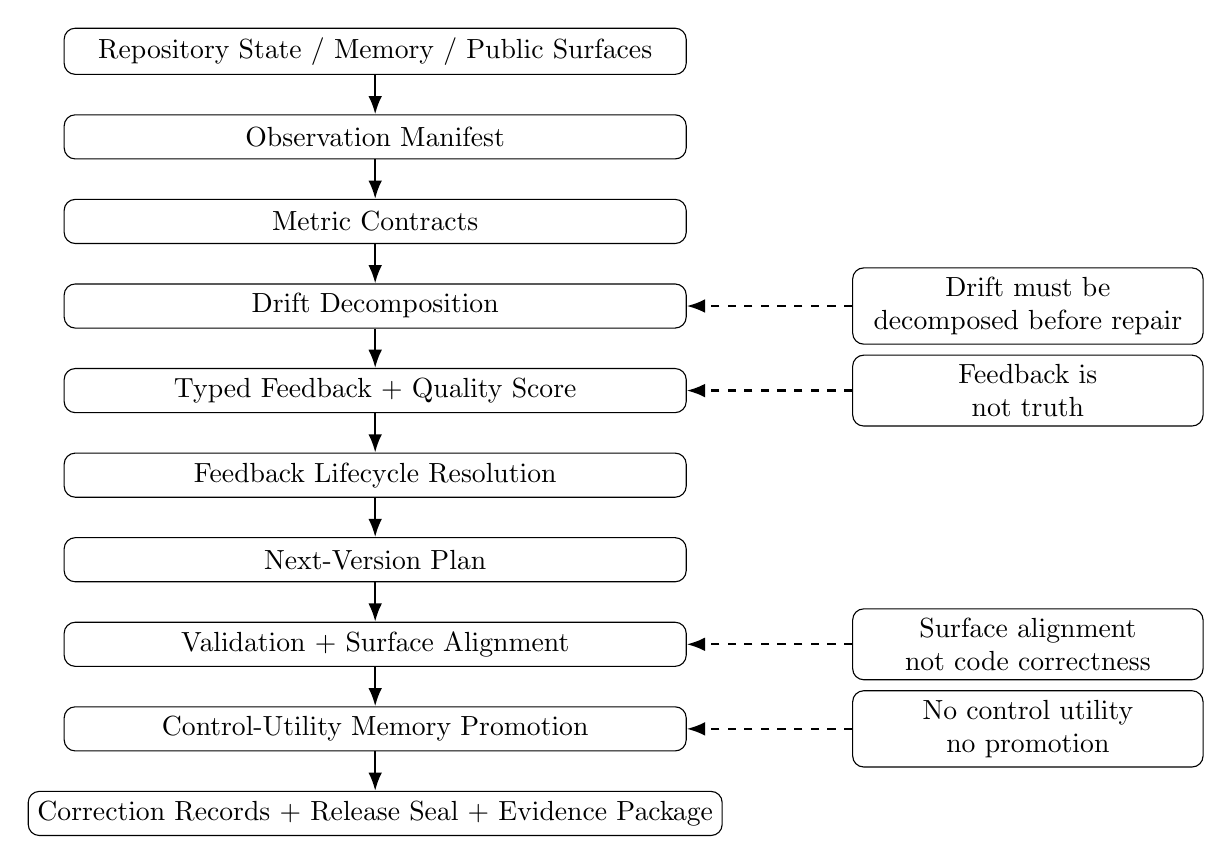
\begin{tikzpicture}[
  node distance=0.50cm,
  box/.style={rectangle, rounded corners, draw, align=center, minimum width=7.9cm, minimum height=0.56cm},
  smallbox/.style={rectangle, rounded corners, draw, align=center, minimum width=4.45cm, minimum height=0.50cm},
  arrow/.style={-Latex, thick}
]

\node[box] (input) {Repository State / Memory / Public Surfaces};
\node[box, below=of input] (observe) {Observation Manifest};
\node[box, below=of observe] (metric) {Metric Contracts};
\node[box, below=of metric] (drift) {Drift Decomposition};
\node[box, below=of drift] (feedback) {Typed Feedback + Quality Score};
\node[box, below=of feedback] (life) {Feedback Lifecycle Resolution};
\node[box, below=of life] (plan) {Next-Version Plan};
\node[box, below=of plan] (validate) {Validation + Surface Alignment};
\node[box, below=of validate] (memory) {Control-Utility Memory Promotion};
\node[box, below=of memory] (release) {Correction Records + Release Seal + Evidence Package};

\draw[arrow] (input) -- (observe);
\draw[arrow] (observe) -- (metric);
\draw[arrow] (metric) -- (drift);
\draw[arrow] (drift) -- (feedback);
\draw[arrow] (feedback) -- (life);
\draw[arrow] (life) -- (plan);
\draw[arrow] (plan) -- (validate);
\draw[arrow] (validate) -- (memory);
\draw[arrow] (memory) -- (release);

\node[smallbox, right=2.1cm of drift] (block1) {Drift must be\\decomposed before repair};
\draw[arrow, dashed] (block1) -- (drift);

\node[smallbox, right=2.1cm of feedback] (block2) {Feedback is\\not truth};
\draw[arrow, dashed] (block2) -- (feedback);

\node[smallbox, right=2.1cm of validate] (block3) {Surface alignment\\not code correctness};
\draw[arrow, dashed] (block3) -- (validate);

\node[smallbox, right=2.1cm of memory] (block4) {No control utility\\no promotion};
\draw[arrow, dashed] (block4) -- (memory);

\end{tikzpicture}
\end{center}

%──────────────────────────────────────────────────────────────────────────────
\section{Roadmap}
%──────────────────────────────────────────────────────────────────────────────

\begin{longtable}{p{0.16\textwidth}p{0.74\textwidth}}
\toprule
\textbf{Version} & \textbf{Goal} \\
\midrule
v0.1 & Architecture, contracts, repository layout, schemas, CLI design, evidence grammar. \\
v0.2 & Minimal runnable observation, metric contracts, and drift-report engine. \\
v0.3 & Feedback quality scoring, lifecycle engine, and next-version planner. \\
v0.4 & Control-utility memory promotion and correction-record ledger. \\
v0.5 & README/RCC/public-surface drift guard and release validator. \\
v0.6 & Baseline utility harness and dashboard-ready evidence package. \\
v1.0 & Stable CMS runtime with tests, example evidence packages, RCC surfaces, and public README. \\
\bottomrule
\end{longtable}

%──────────────────────────────────────────────────────────────────────────────
\section{Practitioner Compression}
%──────────────────────────────────────────────────────────────────────────────

CMS-SA v0.1 in practice:

\begin{lstlisting}
1. Observe repository state.
2. Load metric contracts.
3. Decompose drift.
4. Generate typed feedback.
5. Score feedback quality.
6. Resolve feedback lifecycle.
7. Build next-version plan.
8. Validate the plan.
9. Score memory candidates.
10. Promote only control-useful memory.
11. Preserve correction records.
12. Audit README/RCC/AI/public surfaces.
13. Compute release admissibility.
14. Emit release seal and evidence package.
15. Downgrade anything that fails.
\end{lstlisting}

Short law:

\[
\boxed{
\text{No metric contract, no improvement claim.}
\quad
\text{No lifecycle, no feedback control.}
}
\]

\[
\boxed{
\text{No control utility, no memory promotion.}
\quad
\text{No surface alignment, no release.}
}
\]

%──────────────────────────────────────────────────────────────────────────────
\section{Concluding Compression}
%──────────────────────────────────────────────────────────────────────────────

CMS-SA v0.1 names the first executable software architecture for Cybernetic
Memory System governance:

\[
\boxed{
\text{Cybernetic Memory System Software Architecture}
}
\]

It preserves the CMS v1.0/v1.1 spine:

\[
\boxed{
Observe
\rightarrow
Measure
\rightarrow
Compare
\rightarrow
Feedback
\rightarrow
Lifecycle
\rightarrow
Plan
\rightarrow
Validate
\rightarrow
Promote
\rightarrow
Release.
}
\]

It injects Codex software governance:

\[
\boxed{
MetricContract
\rightarrow
DriftReport
\rightarrow
FeedbackLifecycle
\rightarrow
ControlUtilityPromotion
\rightarrow
EvidencePackage.
}
\]

Its first valid runtime targets are:

\[
\boxed{
cms\text{-}lite\text{-}self\text{-}audit
\quad
readme\text{-}rcc\text{-}drift
\quad
feedback\text{-}lifecycle
\quad
memory\text{-}promotion
\quad
baseline\text{-}utility
\quad
public\text{-}surface\text{-}drift.
}
\]

Its first admissibility score is:

\[
\boxed{
\mathcal{A}_{CMS}
=
B_sB_mB_dB_fB_lB_pB_vB_uB_cB_aB_{pub}B_r(1-O).
}
\]

Its first valid maturity claim is conservative:

\[
\boxed{
CMS\text{-}SA\ v0.1
\Rightarrow
\text{architecture-only until a runnable repository and evidence package exist.}
}
\]

The software law is:

\[
\boxed{
\text{No metric contract, no improvement claim.}
\quad
\text{No validation, no release.}
\quad
\text{No control utility, no memory promotion.}
}
\]

The non-claim lock remains:

\begin{center}
\fbox{\begin{minipage}{0.90\textwidth}
\centering
Feedback is not truth.\quad Memory is not consciousness.\quad Surface alignment is not code correctness.
\end{minipage}}
\end{center}

Thus CMS-SA v0.1 evolves CMS from a source-bounded cybernetic-memory theory into
a software architecture ready for implementation. It preserves the CMS v1.0/v1.1
source boundary, injects Codex evidence governance, and begins with the smallest
useful implementation: a runnable repository-memory control system that emits
observations, metric contracts, drift reports, feedback lifecycle records,
next-version plans, validation reports, control-utility memory decisions,
correction records, surface-alignment audits, release seals, and evidence
artifacts.

\end{document}